% !TEX root = bipartite.tex

\section{Edge weighting using \emph{tf-idf}} \label{sec:tfidf}

One of the most common methods used in information retrieval is the \emph{term
frequency -� inverse document frequency} (or \emph{tf--idf}), a weighing scheme
for quantifying the importance of a term to a document in a collection
\citep{salton1988term}. The tf--idf weight is assigned to each term-document
pair and is proportional to the relative frequency of the word in the document,
adjusted by the proportion of that word over the entire collection. This method
and variations of it are used by search engines as a central component for
ranking the relevance of a document to a query, but also in other applications
like text summarization and classification.

The tf--idf weight of a term $t$ for a document $d$ in a collection $D$ is
defined as the product of the term frequency and inverse document frequency:

\begin{equation}
\label{formula:tfidf}
w_d(t) = f_d(t) \times log(\frac{\mid D\mid}{|\{d \in D : t \in d\}|})
\end{equation}

The term frequency $f_d(t)$ in equation \ref{formula:tfidf} can be the raw or
relative frequency of the term $t$ in the document $d$. The inverse document
frequency (second part of the product) measures whether the term is common or
rare across all documents in the collection $D$ and is calculated by taking the
logarithm of the fraction of the size of the collection $D$ to the number of
documents containing the term $t$.

We propose a similar approach for (re)weighting a user-object bipartite network
in order to reduce the impact of highly popular objects on projection and
clustering. Let us replace the documents in the tf--idf scheme with users and
terms with objects, and define a weighting scheme as below:

\begin{equation}
\label{formula:weight}
w_{new}(u,o) = f(u,o) \times
log(\frac{|U|}{d(o)})
\end{equation}

The new weight (\ref{formula:weight}) of an edge between an user and an object
can be recalculated as the product of the normalized object frequency and the
logarithm of the inverse object frequency across all users. The former
represents the number of object-user interactions (edge weight) with some
normalization technique applied. Normalization is required to prevent a bias
towards more active users. For example one can normalize the weight of an edge
between an user and an object by taking the ratio of its value to the maximum
weight of any given edge connected to that user (\ref{formula:tfmax}).

\begin{equation}
\label{formula:tfmax}
f(u,o) = \frac{w(u,o)}{max\{w(u,p) : p \in N(u)\}}
\end{equation}

The last part of the product in equation \ref{formula:weight} is similar to the
concept of \emph{inverse document frequency} and measures whether the object is
common or rare across all users. It is calculated by dividing the total number
of users by the (unweighted) degree of the object (number of users interacting
with the object), and taking the logarithm of this value.

The re-weighting scheme presented above assigns higher values to frequent
interactions between users and objects offset by how popular an object is within
the collection of users. Unpopular objects increases the weight of an
interaction while very popular ones make the interaction less significant.

Once the new weights have been calculated, thresholding can be applied to filter
out irrelevant edges. As we'll see in section \ref{sec:eval}, this reduces
significantly the edge inflation in the projected networks while increasing the
quality of partitions resulted from community detection and improving the
performance of the algorithms.

\begin{figure}[t] \centering
  \begin{tabular}{cc} 
    \subfloat[Example network with tf-idf
  weights]{\label{fig:example_weighted_tfidf}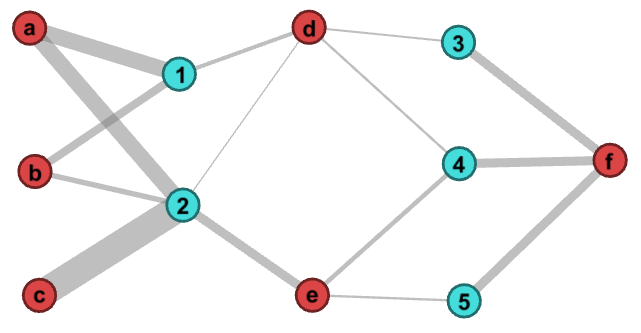
\includegraphics[width=6cm]{./figures/example_weighted_tfidf.png}}
  & \subfloat[Filtered network $\tau =
  0.3$]{\label{fig:example_filtered}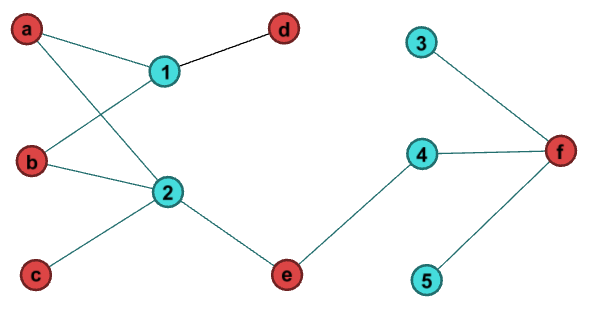
\includegraphics[width=6cm]{./figures/example_rm_weighted.png}}
  \end{tabular}
  \caption{Example of user-object network with \emph{tf-idf} weighting and
  filtering applied}
  \label{fig:example_all}
\end{figure}

Figure \ref{fig:example_all} illustrates the network example from section
\ref{sec:ubnetworks} (figure \ref{fig:example}) with the proposed \emph{tf-idf}
method applied. Weights are assigned to edges based on their initial value and
transformed through equation \ref{formula:weight}. In our example they vary
between 0.1 and 2.3. The thickness of an edge is proportional to the resulted
weight after \emph{tfidf} is applied. As illustrated in figure
\ref{fig:example_weighted_tfidf}, the lowest values are assigned to edges
pointing at the highest degree object $d$. This object is connected to four out
of five users. The highest weights are assigned to edges connecting users to
unpopular or local objects, for example $a$ and $b$. The initial weight is
also taken into consideration with higher weights assigned to edges having
higher initial value. In our example, edge $1d$ has higher \emph{tfidf} weight
than $2d$, even though both edges end in the same node $d$.

After filtering out all edges with weights smaller than a threshold (in this
case $\tau = 0.3$), the resulted network has a simpler and more intuitive
structure, containing only relevant edges (figure \ref{fig:example_filtered}).
In the next section, we will validate the proposed approach and confirm this
observation on large real-world networks.
